\documentclass{article} % For LaTeX2e
\usepackage{cos424,times}
\usepackage{hyperref}
\usepackage{url}
\usepackage{graphicx}
\usepackage{amsmath}
\usepackage{multirow}
\usepackage{caption}
\usepackage{subcaption}

\bibliographystyle{plos2009}

\title{Spam Classification}

\author{Curtis Belmonte\\
{\tt\small curtislb@princeton.edu}
\and
Dorothy Chen\\
{\tt\small dschen@princeton.edu}
}

\newcommand{\fix}{\marginpar{FIX}}
\newcommand{\new}{\marginpar{NEW}}

\begin{document}

\maketitle

\begin{abstract}
Spam, or unsolicited email, is becoming an increasingly large problem as email becomes more and more popular. In this assignment, we discuss various machine learning methods and use them to create spam classifiers. We then analyze the results and effectiveness of these methods. We found that logistic regression is the best method to use for this problem, and AdaBoost is the least preferable. 
\end{abstract}

%------------------------------------------------------------------------
\section{Introduction and background}
Email is something used daily by a large number of people. Advertisers and other people trying to sell things have taken advantage of this fact by sending out unsolicited emails, which is referred to as spam. In response to this, spam filters were created to identify these emails and to keep them from clogging up inboxes.

%------------------------------------------------------------------------
\section{Description of data and data processing}
The training data set consists of 22,500 spam and 22,500 non-spam emails from the trec07p data set. We used the provided script to define a vocabulary and create a bag-of-words representation for each email. The resulting vocabulary contained 9579 words. The classifiers are built using these bag-of-words representations as features for the training data. The testing data set consists of 2,500 spam and 2,500 non-spam emails from the same corpus, and they are processed in a similar manner to also create bag-of-words representations. 

We also used 180,000 emails from the Enron data set [3] and used it for testing across data sets. 

%------------------------------------------------------------------------
\section{Methods}
We used the methods implemented in the scikit-learn package. [1]
\subsection{Simple methods}
\begin{enumerate}
  \item Naive Bayes classifier, using multinomial implemenation
  \item Decision tree, using Gini impurity scores and no max tree depth
  \item Logistic regression, with $l_2$ penalty
\end{enumerate}

\subsection{Complex methods (ensemble learning)}
\begin{enumerate}
  \item Random forests, with 10 trees and Gini impurity scores 
  \item AdaBoost, with 50 decision stumps as weak learners
\end{enumerate}

%------------------------------------------------------------------------
\section{Analysis of results}
\subsection{Evaluation metrics}
For each classification method, we used stratified 5-fold cross-validation on the training set of emails. We used the same number of folds across all methods in order to facilitate comparison.

Preliminary comparison of results, was done using accuracy and ROC curves. The ROC curve for multinomial naive Bayes can be seen in figure \ref{fig:nb}(a) and indicates a high true positive and low false positive rate. The precision-recall curve can be seen in figure \ref{fig:nb}(b) and also shows that this classifier has extremely good performance. Curves for our other methods looked extremely similar to these, so they are not included in this report. The full set of ROC and precision-recall curves can be found in the ``writeup/images'' folder of the GitHub repository for this project. [2] In an effort to view the data more clearly, we plotted the data on log scales. Specifically, we plotted the x-axis on a log10 scale in order to examine lower false positive rates. However, this did not significantly change the quality of the graph so we decided not to include them.

\begin{figure}[h]
  \centering
  \begin{subfigure}{0.35\textwidth}
    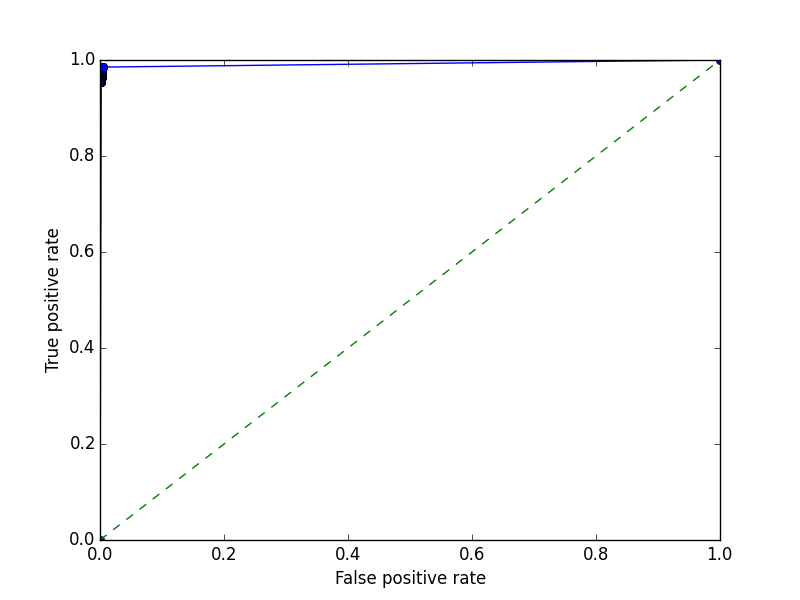
\includegraphics[width=\textwidth]{images/naive_bayes_roc_curve.png}
    \caption{ROC curve}
  \end{subfigure}
  \begin{subfigure}{0.35\textwidth}
    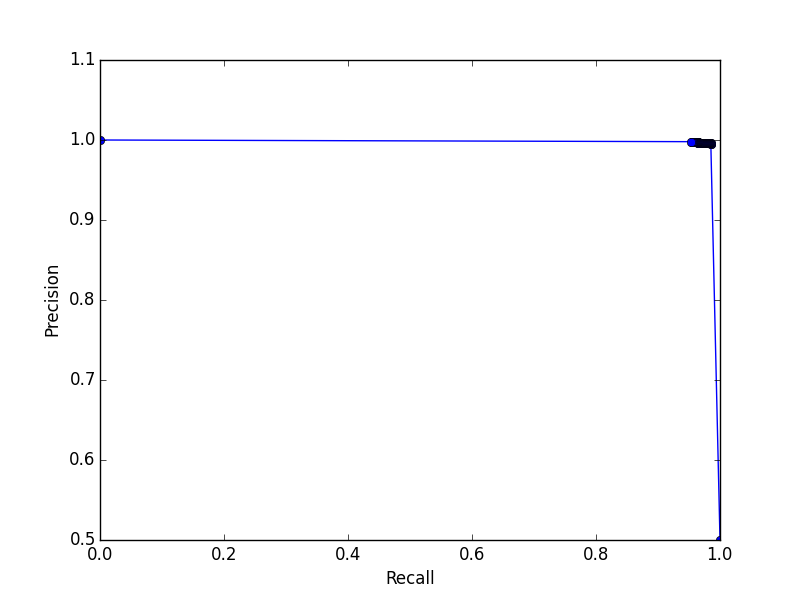
\includegraphics[width=\textwidth]{images/naive_bayes_pr_curve.png}
    \caption{Precision-recall curve}
  \end{subfigure}
  \caption{ROC and precision-recall curves for Multinomial Naive Bayes}
  \label{fig:nb}
\end{figure}

We then did further analysis and comparison using precision, recall, and $F_1$ scores. In figure \ref{fig:table}, we can see values for the methods run on both the entire corpus at once and for averages from running 5-fold cross-validation. 

There are a few differences between running classifiers on the entire corpus versus doing cross-validation. The most easily explained of these is the time: because cross-validation trains using 4/5 of the available data, it will take less time than training on all the data. 

\begin{figure}[h]
  \begin{tabular}[h]{ | c | c | r | r | r | r | r | }
    \hline
    Classifier    &                  & Time (s) & Accuracy & Precision & Recall & $F_1$ score  \\ \hline
    Naive Bayes   & Entire data set  & 1.51     & 0.9874   & 0.9963    & 0.9784 & 0.9873 \\ \cline{2-7}
                  & Cross-validation & 1.25     & 0.9940   & 0.9984    & 0.9895 & 0.9939 \\ \hline
    Decision Tree & Entire data set  & 150.0    & 0.9948   & 0.9950    & 0.9936 & 0.9947 \\ \cline{2-7}
                  & Cross-validation & 106.05   & 0.9856   & 0.9956    & 0.9752 & 0.9850 \\ \hline
    Logistic Regr & Entire data set  & 8.62     & 0.9974   & 0.9996    & 0.9952 & 0.9974 \\ \cline{2-7}
                  & Cross-validation & 6.08     & 0.9968   & 0.9955    & 0.9981 & 0.9968 \\ \hline
    Random Forest & Entire data set  & 11.46    & 0.9968   & 0.9992    & 0.9944 & 0.9968 \\ \cline{2-7}
                  & Cross-validation & 8.18     & 0.9976   & 0.9969    & 0.9984 & 0.9976 \\ \hline
    AdaBoost      & Entire data set  & 642.94   & 0.9916   & 0.9976    & 0.9856 & 0.9915 \\ \cline{2-7}
                  & Cross-validation & 482.88   & 0.9966   & 0.9970    & 0.9962 & 0.9966 \\ \hline
  \end{tabular}
  \caption{Results from using various methods}
  \label{fig:table}
\end{figure}

\subsection{Running time}
As we can see in figure \ref{fig:table}, using Naive Bayes is by far the fastest of the five methods we used. Logistic regression and random forests perform reasonably well. Decision trees, however, are rather slow. This is due to the fact that we did not constrain the height of the tree. AdaBoost is prohibitively slow and does not offer any sort of increase in performance with regards to accuracy. It is therefore a suboptimal choice for solving this problem. 

\subsection{Feature selection results}
We tried selection of 5, 10, and 15\% of features. Performance among the three was best at the 5\% level of selection; we have included these results in figure \ref{fig:table_selected}. In comparison to learning on the entire training set, performance on the feature selected set in terms of accuracy, precision, recall, and $F_1$ decreased slightly. On the other hand, running time also decreased dramatically for most methods.  

An exception to the running time decreasing drastically is logistic regression. While its running time decreased after feature selection, it does not scale linearly with the number of features. For example, the running time for naive Bayes dropped from 1.51 to 0.08 seconds (about 5\% of its original runtime) after feature selection. In contrast, the running time for logistic regression only dropped from 8.62 to 6.01 (69.7\% of its original runtime). 

Because the drop in correctness is most likely not as significant as the boost in performance time-wise in most situations, feature-selected training and testing is probably preferable. In situations that require high accuracy/precision, however, using the full feature set would still be better. 

\begin{figure}[h]
  \begin{tabular}[h]{ | c | c | r | r | r | r | r | }
    \hline
    Classifier    &                  & Time (s) & Accuracy & Precision & Recall & $F_1$ score  \\ \hline
    Naive Bayes   & Entire data set  & 0.08     & 0.9526   & 0.9752    & 0.9288 & 0.9514 \\ \cline{2-7}
                  & Cross-validation & 0.07     & 0.9629   & 0.9636    & 0.9632 & 0.9630 \\ \hline
    Decision Tree & Entire data set  & 2.96     & 0.9936   & 0.9952    & 0.9920 & 0.9936 \\ \cline{2-7}
                  & Cross-validation & 2.19     & 0.9925   & 0.9956    & 0.9894 & 0.9925 \\ \hline
    Logistic Regr & Entire data set  & 6.01     & 0.9938   & 0.9968    & 0.9908 & 0.9938 \\ \cline{2-7}
                  & Cross-validation & 3.13     & 0.9954   & 0.9954    & 0.9954 & 0.9954 \\ \hline
    Random Forest & Entire data set  & 0.82     & 0.9972   & 0.9984    & 0.9960 & 0.9972 \\ \cline{2-7}
                  & Cross-validation & 0.60     & 0.9976   & 0.9972    & 0.9981 & 0.9976 \\ \hline
    AdaBoost      & Entire data set  & 26.26    & 0.9868   & 0.9959    & 0.9776 & 0.9867 \\ \cline{2-7}
                  & Cross-validation & 17.88    & 0.9956   & 0.9965    & 0.9947 & 0.9956 \\ \hline
  \end{tabular}
  \caption{Results from using various methods after performing feature selection}
  \label{fig:table_selected}
\end{figure}

\subsection{Important features}
During feature selection, we selected the ``best'' 5\% of features. Features were ranked by statistical significance, which was found using ANOVA analysis. We looked at the top 20 features according to this analysis, and most of the words appeared to be part of email headers. Some examples include: ``unsubscrib'', ``list'', ``bounce'', ``subject'', and ``mailto''. This suggests that a possible extension is examining these email headers more closely. Two of our features are actually ``spam'' and ``spamassassin'', suggesting that these emails have already been classified at least once or are announcing themselves as ``not-spam''. This may have impacted our performance on this data set. 

\subsection{False negatives versus false positives}
For the problem of spam classification, it's better to have false negatives than false positives. This is because a user can manually specify that an email is spam, but they are unlikely to explore their ``spam'' folder. Therefore, non-spam emails classified as spam are likely to be missed entirely; this is highly undesirable. In general, the added hassle of having to deal with an occasional spam email outweighs the cost of missing an important email. 

\subsection{Hard cases to classify}
We considered an example ``hard'' to classify if it was misclassified by more than one classifier. Hard false positives were rare, but appear to mostly be emails send to mailing lists.

The only cases that were misclassified by all of our classifiers were false negatives. Hard examples included emails whose entire bodies consisted of random strings of letters (commonly text representations of images). Because we used a bag-of-words representation, it would treat these long strings as unique. Many other examples were very short emails. It makes sense that these might be misclassified because there's just not that much content to work with. Finally, one spam email was written entirely in German, which the classifiers did not catch because most, if not all, of the other emails in this data set were written in English. 

%------------------------------------------------------------------------
\section{Generalization across datasets}
We trained a logistic regression classifier on the trec07p training data and tested it on the Enron data set. The results are summarized in figure \ref{fig:table_comparison}. The classifiers did much worse than they did when we tested it on the trec07p set. This indicates that the classifiers instead learned data set-specific features rather than general spam-specific features. 

Feature selection did not help at all and actually decreased performance. While feature selection is intended to increase performance by decreasing overfitting, that did not happen in this case. This might be because the ``best'' features that were chosen could all have been data set-specific features, which would actually increase overfitting and explain the decrease in performance. 

\begin{figure}[h]
  \begin{tabular}[h]{ | c | c | r | r | r | r | r | }
    \hline
    Classifier    & Feature selection? & Time (s) & Accuracy & Precision & Recall & $F_1$ score  \\ \hline
    Naive Bayes   & No                 & 1.46     & 0.6691   & 0.7610    & 0.4930 & 0.5984       \\ \cline{2-7}  
                  & Yes                & 0.08     & 0.4876   & 0.4847    & 0.3922 & 0.4336       \\ \hline
    Logistic Regr & No                 & 8.48     & 0.4076   & 0.4426    & 0.7126 & 0.5460       \\ \cline{2-7}
                  & Yes                & 5.88     & 0.3147   & 0.3811    & 0.5939 & 0.4643       \\ \hline
  \end{tabular}
  \caption{Results from using classifiers trained on trec07p and testing on the Enron data set}
  \label{fig:table_comparison}
\end{figure}

%------------------------------------------------------------------------
\section{Conclusion and possible extensions}

For the problem of spam classification, logistic regression seems to be the best choice to use of the five methods we explored. It had extremely high accuracy, precision, and recall and also had reasonable running time. Furthermore, its running time scales sublinearly with respect to the number of features. AdaBoost is not a good choice for this problem due to its large running time and its lack of increased performance relative to other possibilities. 

Feature selection presents a tradeoff between correctness and computational time, but correctness suffers by a far smaller margin than computational time is benefited. In time-sensitive situations, using feature selection would definitely be preferable; in general, feature selection is probably still preferable.

We feel that using a different model to represent the emails' content would be an interesting and potentially useful extension. While the bag-of-words model was certainly effective, many features were lost; in particular, we feel that things such as word order, capitalization, and punctuation are especially important in language and that their exclusion may have negatively impacted performance. Word order is important because it encodes meaning and context of sentences--single words on their own may be ambiguous. This could be accomplished using a bigram model, as discussed by Cormack et al (2007) [4]. Capitalization also matters, as emails in all capitals, for example, are probably more likely to be spam. Punctuation matters because emails with punctuation are more likely to have proper grammar, and correct grammar intuitively seems indicative of non-spam (or, at least non-computer generated) emails. 

One other feature is looking for attachments on files and possibly also looking at their types/file extensions. This would help solve the issue we ran into with image attachments that ended up being spam but were missed by our classifier. 

It also may be beneficial to compare the words we get to actual English words. This would help remedy the issue with missing spam emails that just consisted of long strings of random letters or that were written in other languages. 

Furthermore, because false positives are worse than false negatives, it may be helpful to penalize false positives more harshly during training to account for this fact. However, some sources, such as Zhang et al (2004), suggest that heavily penalizing false positives may actually reduce performance in some cases. [5]

%------------------------------------------------------------------------
\section{References}
\bibliography{ref}
[1] Pedregosa F, Varoquaux G, Gramfort A, Michel V, Thirion B, et al. (2011) Scikit-learn: Machine learning in Python. Journal of Machine Learning Research 12: 2825–2830.

[2] https://github.com/curtislb/SpamClassifier

[3] Bryan Klimt and Yiming Yang. Introducing the enron corpus. In CEAS, 2004.

[4] G. V. Cormack, G. Hidalgo, E. P. Sánz, and J. María. Spam Filtering for Short Messages. In CIKM, 2007.

[5] Le Zhang, Jingbo Zhu, and Tianshun Yao. An evaluation of statistical spam filtering techniques. ACM Transactions on Asian Language Information Processing (TALIP) volume 3 issue 4: 243-269, 2004.

\end{document}
